\documentclass[12pt]{article}

\usepackage[a4paper,top=3cm,bottom=2cm,left=2cm,right=2cm,marginparwidth=1.2cm]{geometry}
\usepackage{fancyhdr}
\usepackage{tikz}
\usetikzlibrary{shapes.geometric, arrows}

\author{Your Name}
\title{Analytic Studies and Sampling Techniques}
\date{}

\tikzstyle{startstop} = [rectangle, rounded corners, minimum width=3cm, minimum height=1cm,text centered, draw=black, fill=red!30]
\tikzstyle{process} = [rectangle, minimum width=3cm, minimum height=1cm, text centered, draw=black, fill=orange!30]
\tikzstyle{arrow} = [thick,->,>=stealth]
\tikzstyle{box} = [rectangle, minimum width=3cm, minimum height=1cm, text centered, draw=black]


\begin{document}
\pagestyle{fancy}
\lhead{STAT110/115 Tutoring Materials}
\rhead{Study Design}

\begin{itemize}
\item \textbf{Purpose of Analytic Studies}: To test hypotheses (quantify population). For example, do government subsidy programs impact the profitability of fisheries? Does IT investment impact productivity in industry? Does a Mediterranean diet impact life expectancy?
\item \textbf{Function of Replication}: To allow us to separate out true effects from chance effects.
\item \textbf{Function of Control}: Provides context for evaluating the effect of interest.
\item \textbf{Descriptive Studies}: The characteristics of people with a disease (person; place; time); lifestyle patterns in a population; attitudes to health care.
\item \textbf{Well-defined and Not Well-defined Population}:
    \begin{itemize}
    \item Well-defined: The collection of words in poems by W. B. Yeats. All patients diagnosed with colorectal cancer in New Zealand in 2015.
    \item Not well-defined: The population of New Zealand. Right now? Past? Future?(Time). Target population for a particular cancer treatment. Which type/stage of cancer? Existing or future patients(time)? Over a certain age? On other medications?
    \end{itemize}
\item \textbf{Traits of Random Sampling}: Known-chance, Equal-chance. If doesn't have those traits, define the sample has representative or not.
\item \textbf{Sampling Frame Definition}: List of all eligible sampling units from which the sample will be drawn. For example, to draw 200 out of 10,000 employees to form a sample, the roster of 10,000 employees, is the sampling frame. May be sourced from census, company data base or other secondary data. Completeness may be an issue when sourcing Sampling Frame. Sometimes need to use/combine multiple sample frames. Non-probability sampling techniques don't require a sampling frame.
\item \textbf{Sources of Error for Sample Mean}:

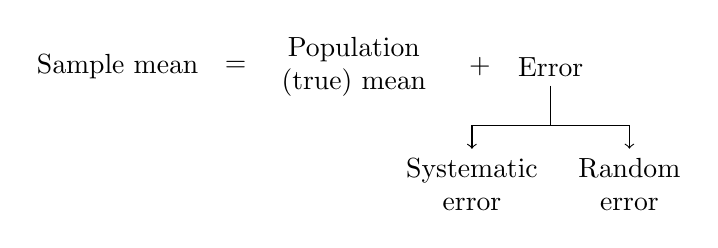
\begin{tikzpicture}
\node (samplemean) at (0,0) {Sample mean};
\node (equals) at (1.5,0) {=};
\node [align=center](populationmean) at (3,0) {Population \\ (true) mean};
\node (plus) at (4.6,0) {+};

\node (error) at (5.5,0) {Error};

\node[below of=error, align=center, xshift=-1cm, yshift=-0.5cm] (systematicerror) {Systematic \\ error};
\node[right of=systematicerror, align=center, xshift=1cm] (randomerror) {Random \\ error};

\draw[->] (error.south) -- ++(0,-0.5)-|  node[near start,below] {}(systematicerror.north);
\draw[->] 	(error.south)-- ++(0,-0.5)-| node[near start,below] {}(randomerror.north);
\end{tikzpicture}

    \begin{itemize}
    \item \textbf{Random Error}: Due to natural variability. Increasing the sample size will reduce the random fluctuations in the sample mean. Statistical methods allow us to quantify the influence of random error on our estimate.
    \item \textbf{Systematic Error in a Descriptive Study (Bias)}: Due to aspects of the design or conduct of the study which systematically distort the results. Occurs if a sample is not representative of the population (Selection bias). Occurs if the information collected from the sample members is incorrect (Information bias). Cannot be reduced by increasing the sample size.
    \end{itemize}
\item \textbf{Probability Sampling}: We want our sampling frame to match the population of interest and provide a way to draw a sample. Probability sampling is important because it helps to justify the statistical models. For a finite population of size N draw a sample of size n such that each possible sample has the same probability of being selected.
\item \textbf{Key Characteristic of Probability Sampling}: The key characteristic is that we know the probability of being selected for everyone in the sample frame.
\item \textbf{Simplest Form of Probability Sampling}: Simple random sampling.
\item \textbf{Types of Probability Sampling}: Simple random sampling, stratified random sampling, cluster sampling.
\item \textbf{Traits of Simple Random Sampling}: Same chance of selection (e.g., Lotto).
\item \textbf{Advantages of Stratified Sampling}: More precise estimate than for the same sample size from a simple random sample. Can take different sized samples from different strata (a device for reducing overall variability). Useful if you are interested in the results for each stratum and some of the strata are small. Example: colon cancer treatment, samples of colon cancer patients, stratified by ethnicity.
\item \textbf{Types of Stratified Sampling}: Proportionate stratified sample, disproportionate stratified sample (equal number from each stratum).
\item \textbf{Cluster Sampling}: The population may be composed of similar and naturally occurring groups. Dividing the population into a group/cluster (then selecting a sample from each cluster).
\item \textbf{Types of Cluster Sampling}: One-stage, two-stage. Pros and cons for two stage cluster sampling: reduce cost \& time, less precise.
\item \textbf{Experimental Studies}: The researcher manipulates the conditions (intervenes in a natural process) and records the results. The aim is to control all other factors to isolate the effects of the intervention. Best way to study causation. Why randomisation? Randomisation can be used to ensure that effects of unmeasured factors are equalised across the intervention and control groups. Why NOT experimental studies? Ethical problems.
\item \textbf{Observational Studies}: The investigator does not intervene, simply observes a naturally occurring process, and collects information. The idea is to get as close as possible to the information that would have been obtained if the experimental study could have been done. Cons: We can't know the confounding factors.
\item \textbf{Case Control Study}: Outcome trace back to reason.
\item \textbf{Traits of Randomised Controlled Trial (RCT)}: 
	\begin{itemize}
	\item Is considered the "gold standard" analytic study.
	\item \textbf{Randomisation} - or random allocation, is used to create two comparable groups, one who will have the placebo treatment and the other the experimental treatment. At the end of follow-up any difference between the groups can be attributed to the difference in treatment.
	\item \textbf{Control group} - is used to isolate the effects of the intervention.
	\end{itemize}
\item \textbf{What is blinding?}: Blinding refers to not knowing whether the participant is in the intervention or the control group. Several people may be blinded to the allocation including the participants, the people caring for patients, the people measuring outcomes, the lead researcher.
\item \textbf{Pros and cons for RCT}:
    \begin{itemize}
    \item Advantages: Experiment - the best way to test an hypothesis. If the trial is well conducted, differences in outcome can be attributed to the intervention.
    \item Disadvantages: May not be ethical or feasible.
    \end{itemize}
\item \textbf{Example cohort study}: British doctors and smoking. Aim: to investigate the relationship between smoking and lung cancer.
\item \textbf{Pros and cons for cohort study}:
    \begin{itemize}
    \item Pros: Clear chronological order from reason to outcome. Can evaluate the relationship between multiple results and factor(s).
    \item Cons: Large time consumption. Bias affect. Small sample size.
    \end{itemize}
\item \textbf{Characteristics of a case-control study}: Generally carried out to test hypotheses. Participants are chosen on the basis of their outcome status: a group with the outcome (cases) and a group without (controls). Information is collected from people with and without outcome about exposures that occurred in the past (retrospective). i.e. in general before disease was diagnosed.
\item \textbf{Pros and cons for Case-control study}:
    \begin{itemize}
    \item Advantages: Relatively quick. Smaller than cohort studies, particularly for rare outcomes. Can examine the effects of multiple exposures.
    \item Disadvantages: Events have already occurred so the potential for bias is higher. It is very hard (if not impossible) to remove all the effects of confounding.
    \end{itemize}
\item \textbf{Sources of error in analytic studies}

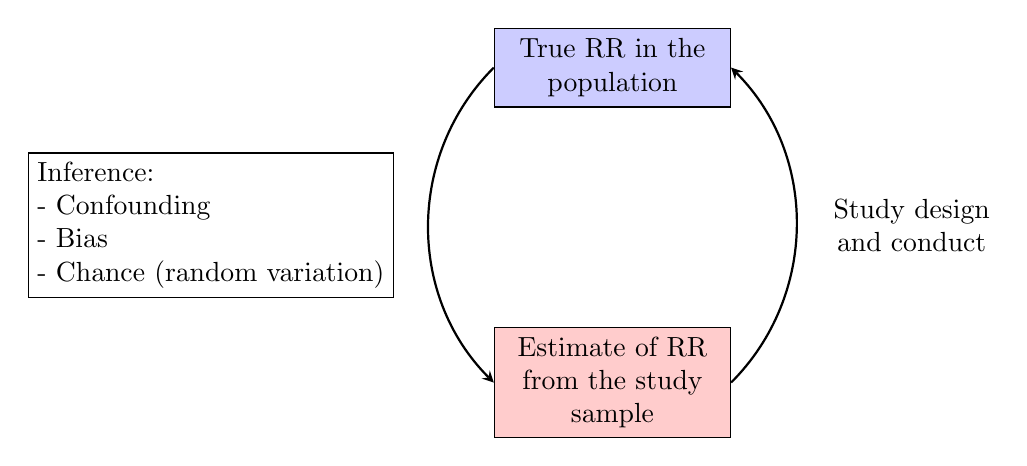
\begin{tikzpicture}[node distance=2cm]
% Nodes
\node (trueRR) [process, align=center, fill=blue!20] {True RR in the \\ population};
\node (estimateRR) [process, align=center, fill=red!20, below of=trueRR, yshift=-2cm] {Estimate of RR \\ from the study \\ sample};
\node (inference) [box, align=left, left of=trueRR, xshift=-3.1cm, yshift=-2cm] {Inference: \\ - Confounding \\ - Bias \\ - Chance (random variation)};
\node (studyDesign) [right of=trueRR, align=center, xshift=1.8cm, yshift=-2cm] {Study design \\ and conduct};
% Arrows
\draw [arrow] (trueRR.west) to [bend right=45] (estimateRR.west);
\draw [arrow] (estimateRR.east) to [bend right=45] (trueRR.east);
\end{tikzpicture}

\item \textbf{What is Confounding?}: Confounding is a distortion of the association between exposure and outcome caused by the presence of a third factor. A confounder is a variable which causes this distortion.
\item \textbf{A variable must be both ( ) to become a confounder}:
    \begin{itemize}
    \item associated with the exposure (independent of outcome);
    \item and associated with the outcome (independent of exposure).
    \end{itemize}
\item \textbf{Bias in an analytic study}:
    \begin{itemize}
    \item \textbf{Selection bias}: arising from the way participants are selected for inclusion in the study. In an analytic study, selection bias occurs if the selection processes cause a systematic difference between the groups of participants selected for the study. Prospective analytic studies rarely obtain participants through random sampling from a population. The issue of representativeness must be considered, but for analytic studies we consider it a generalisability issue rather than bias.
    \item \textbf{Information bias}: arising from the way study information is obtained, interpreted and recorded. In an analytic study, information bias is a particular problem if there are systematic differences in the information obtained from groups under comparison in the study. Information bias may be introduced by the observer, the study individual (respondent), instruments used to collect the data (e.g., badly-designed questionnaire), or missing measurements (e.g., from loss to follow-up in a prospective study).
    \end{itemize}
\item \textbf{RCT, Cohort study, Case-control study}:
    \begin{itemize}
    \item \textbf{Randomised controlled trial}: Analytic, experimental, prospective.
    \item \textbf{Cohort study}: Analytic, observational, usually prospective.
    \item \textbf{Case-control study}: Analytic, observational, retrospective.
    \end{itemize}
\item \textbf{Summary for the classification}:

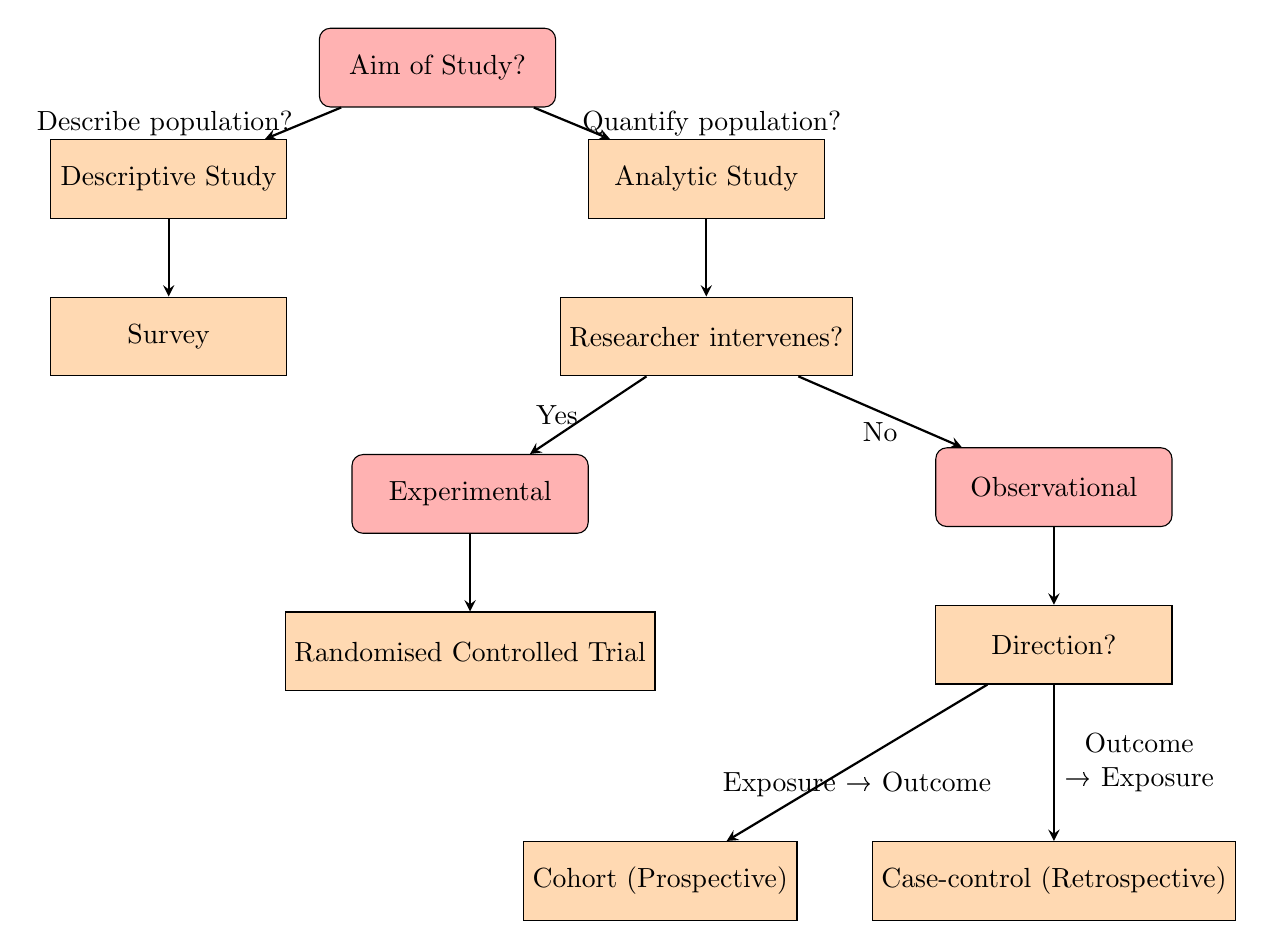
\begin{tikzpicture}[node distance=2cm]

\node (study) [startstop] {Aim of Study?};
\node (desc) [process, below left of=study, xshift=-2cm] {Descriptive Study};
\node (analytic) [process, below right of=study, xshift=2cm] {Analytic Study};
\node (survey) [process, below of=desc] {Survey};
\node (inter) [process, below of=analytic] {Researcher intervenes?};
\node (exp) [startstop, below of=inter, xshift=-3cm] {Experimental};
\node (obs) [startstop, below right of=inter, xshift=3cm, yshift=-0.5cm] {Observational};
\node (rct) [process, below of=exp] {Randomised Controlled Trial};
\node (dir) [process, below of=obs] {Direction?};
\node (cohort) [process, below of=dir, yshift=-1cm] {Case-control (Retrospective)};
\node (casecontrol) [process, left of=cohort, xshift=-3cm] {Cohort (Prospective)};

\draw [arrow] (study) -- node[anchor=east] {Describe population?}(desc);
\draw [arrow] (study) -- node[anchor=west] {Quantify population?}(analytic);
\draw [arrow] (desc) -- (survey);
\draw [arrow] (analytic) -- (inter);
\draw [arrow] (inter) -- node[anchor=east] {Yes} (exp);
\draw [arrow] (inter) -- node[anchor=north] {No} (obs);
\draw [arrow] (exp) -- (rct);
\draw [arrow] (obs) -- (dir);
\draw [arrow] (dir) -- node[anchor=west, align=center] {Outcome \\ → Exposure} (cohort);
\draw [arrow] (dir) -- node[anchor=north] {Exposure → Outcome} (casecontrol);

\end{tikzpicture}

    \begin{itemize}
    \item \textbf{Discrete}: A type of variable that can only take on specific values. These values are typically whole numbers or counts and cannot be subdivided further. For example, the number of children in a family is a discrete variable because it can only be a whole number (e.g., 1, 2, 3, etc.).
    \item \textbf{Categorical}: Represent data that falls into specific categories or groups. The categories in nominal variables do not have any inherent order or ranking. Examples of nominal variables include gender (e.g., male, female), eye colour (e.g., blue, brown, green), or types of fruit (e.g., apple, banana, orange).
    \item \textbf{Continuous}: Measurements that can take on any value within a specific range. They can be subdivided infinitely, and there are no gaps or interruptions in the possible values. Examples of continuous variables include height, weight, temperature, and time. These variables are often represented by real numbers and can include decimal values.
    \item \textbf{Ordinal}: Similar to categorical variables, but they have an inherent order or ranking associated with their categories. The order represents the relative magnitude or importance of the categories, but the actual differences between the categories may not be uniform or measurable. Examples of ordinal variables include educational attainment (e.g., high school, bachelor's, master's, Ph.D.), socioeconomic status (e.g., low, medium, high), or survey ratings (e.g., strongly agree, agree, neutral, disagree, strongly disagree).
    \item \textbf{If a data set is Categorical, must it also be Nominal?}: No. All nominal data is categorical data, but not all categorical data is nominal data. Nominal data refers specifically to categorical data without any order or hierarchy.
    \end{itemize}
\item \textbf{Types of data}


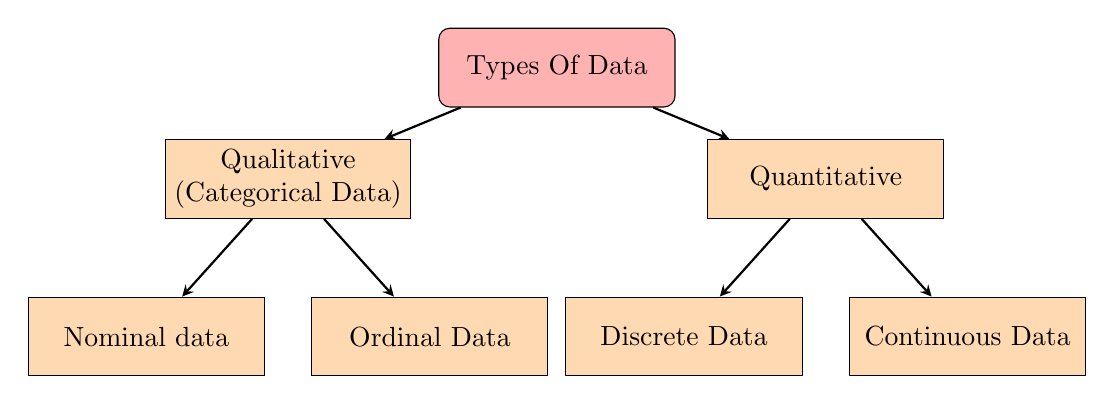
\begin{tikzpicture}[node distance=2cm]

\node (start) [startstop] {Types Of Data};
\node (cat) [process, align=center, below left of=start, xshift=-2cm] {Qualitative \\ (Categorical Data)};
\node (quant) [process, below right of=start, xshift=2cm] {Quantitative};
\node (nominal) [process, below of=cat, xshift=-1.8cm] {Nominal data};
\node (ordinal) [process, below of=cat, xshift=1.8cm] {Ordinal Data};
\node (discrete) [process, below of=quant, xshift=-1.8cm] {Discrete Data};
\node (continuous) [process, below of=quant, xshift=1.8cm] {Continuous Data};

\draw [arrow] (start) -- (cat);
\draw [arrow] (start) -- (quant);
\draw [arrow] (cat) -- (nominal);
\draw [arrow] (cat) -- (ordinal);
\draw [arrow] (quant) -- (discrete);
\draw [arrow] (quant) -- (continuous);

\end{tikzpicture}

\item \textbf{How to identify whether a study uses probability sampling?}: To find sampling frame.
\item \textbf{Note for Stratified sampling}: Stratified sampling involves dividing the population into distinct subgroups (strata) based on certain characteristics.
\item \textbf{Why Non-response can cause bias in surveys?}: because non-respondents tend to(maybe) behave differently compared to people who respond.
\end{itemize}
\end{document}
